%%%%%%%%%%%%%%%%%%%%%%%%%%%%%%%%%%%%%%%%%%%
%%%%%%%%%%%%%%%%%%%%%%%%%%%%%%%%%%%%%%%%%%%
%%%%%%%%%%%%%%%%%%%%%%%%%%%%%%%%%%%%%%%%%%%
\chapter{Introduction}
\label{Sec:Intro}
Proteins are highly complex macromolecules that are vital to biochemical processes taking place in each living organism. Weather alone or as a part of multi-unit complexes, they facilitate vast field of functions such as catalysing chemical reactions, transporting molecules across the cells or replication of DNA. In these processes the ability of a protein to interact with other molecules plays a defining role. 

Since the proper understanding of protein interactions contributes to advances in medicine, pharmaceutics or even agriculture, the study of interaction patterns of proteins has been at the forefront of biochemical research for decades. Unfortunately, the complexity of protein structures and the necessity for expensive and time consuming in-vitro experiments make the progress in the area slow. Many computational tools aim to support this research by simulating the experiments in-silico and thus reducing the costs. However, these tools can produce a vast amounts of data. For example molecular dynamics simulations can mimic the movement of millions of atoms over a given period of time. It is virtually impossible to identify significant patterns by simply observing such simulation. Another example are the protein-protein docking simulations that predict the possible ways two or more proteins interact together. Here the output often comprises of tens to hundreds of possible conformations that the domain expert needs to analyse individually one by one.

Therefore, visualization and visual analysis tools became inherent part of proteomic research both as guidance during the experiments as well as for validation and analysis of results by the domain experts.  The main aim of these tools is to speed up the analysis process by - often interactively - extracting the important features of the data and conveying them in such way, that previously hardly observable patterns and relationships become more prominent. Although much has been done in the field of molecular visualization in the past decades, there are still areas and problems that are not currently addressed. 

%Particularly the area of protein-protein interactions remains largely untouched by scientific literature in terms of visual analysis. 

In this work I will present the current state of the art techniques in the analysis of intermolecular interactions of proteins. I will identify the unsolved problems occurring in the literature, then present the proposed solutions and results that have already been achieved. I will also outline the possibilities for further research.



\chapter{Biochemical Definitions}
\label{Sec:Chem}
Although this thesis deals with the research in the field of visualization and visual analysis, it also ventures into the field of biochemistry. It is therefore inevitable to clarify the basic biochemical terms that will occur throughout the thesis and are important for its proper understanding. This section shall provide the reader with all the necessary knowledge.

\section{Protein Structures}
Proteins are complex molecules formed by one or more chains of amino acids. Amino acids are basic building blocks of all living organisms. There are approximately 500 known amino acids, but only 20 standard amino acids are encoded in genetic code. Each of them consists of \textit{carboxyl group} ($-COOH$), an \textit{amino group} ($-NH_2$) and a unique \textit{side chain} ($-R$) that defines its properties. The three groups are connected by a carbon atom, also called an \textit{alpha carbon} $C_\alpha$. See figure \ref{Fig:aa} a).

\begin{figure}[H]
  \centering
  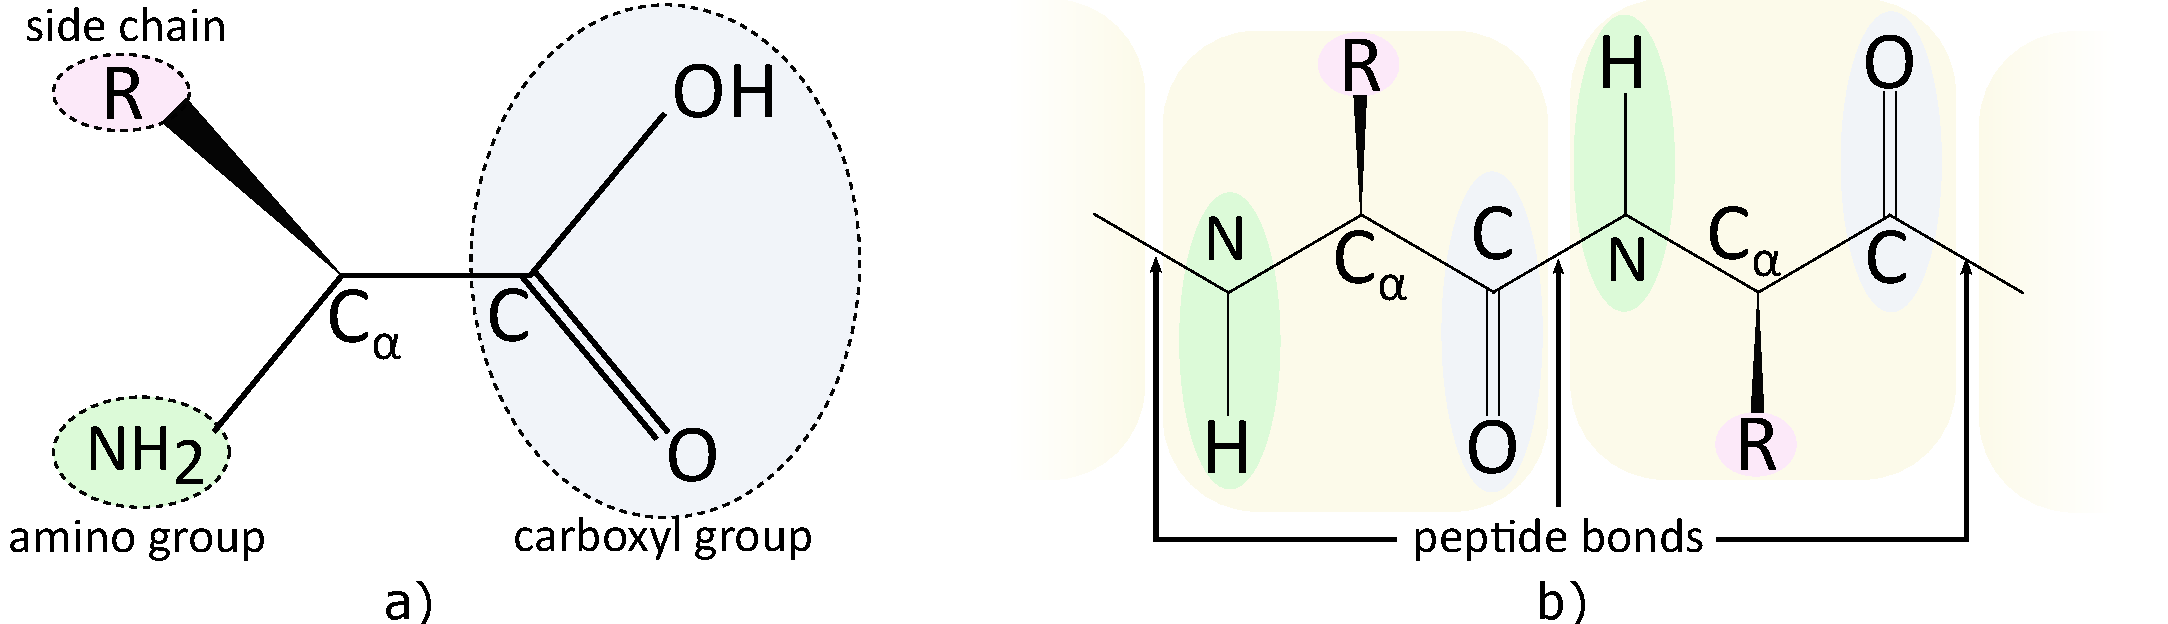
\includegraphics[width=\textwidth]{pictures/aminoacid.pdf} 
  \caption{a) Illustration of a basic amino acid structure. b) Amino acid residues connected into polypeptide chain. It can be noted, that the amino and carboxyl groups are missing atoms, which were released during the formation of peptide bonds as $H_2O$ molecules.}
  \label{Fig:aa}
\end{figure}

During a protein synthesis amino acids are joined together by peptide bonds (covalent bonds), forming polypeptide chains. A peptide bond is formed in a reaction between carboxyl group of one amino acid and amino group of another amino acid (see figure \ref{Fig:aa} b)). As both groups loose atoms that are released as molecule of water during this reaction, the amino acids bonded in polypeptide chains are refereed to as \textit{amino acid residues}. 

Each protein contains at least one long polypeptide chain. This sequence of amino acids, connected by rigid peptide bonds, also known as \textit{backbone}, forms \textit{primary structure} of the protein.

Unlike the peptide bonds, the bonds linking the carboxyl and amino groups to the alpha carbon are free to rotate. Based on these rotations and the patterns of hydrogen bonds that form between hydrogen from amino group and oxygen from corboxyl group, the segments of polypeptide chain can take on various 3D formations. The two most common of those are $\alpha-helices$ and $\beta-sheets$, which are formed by laterally connected $\beta-strands$. These local formations of polypeptide chain are called \textit{secondary protein structures}. Parts of polypeptide chain with absent secondary structures are called \textit{random coils}. See figure \ref{Fig:secondary}.

\begin{figure}[H]
  \centering
  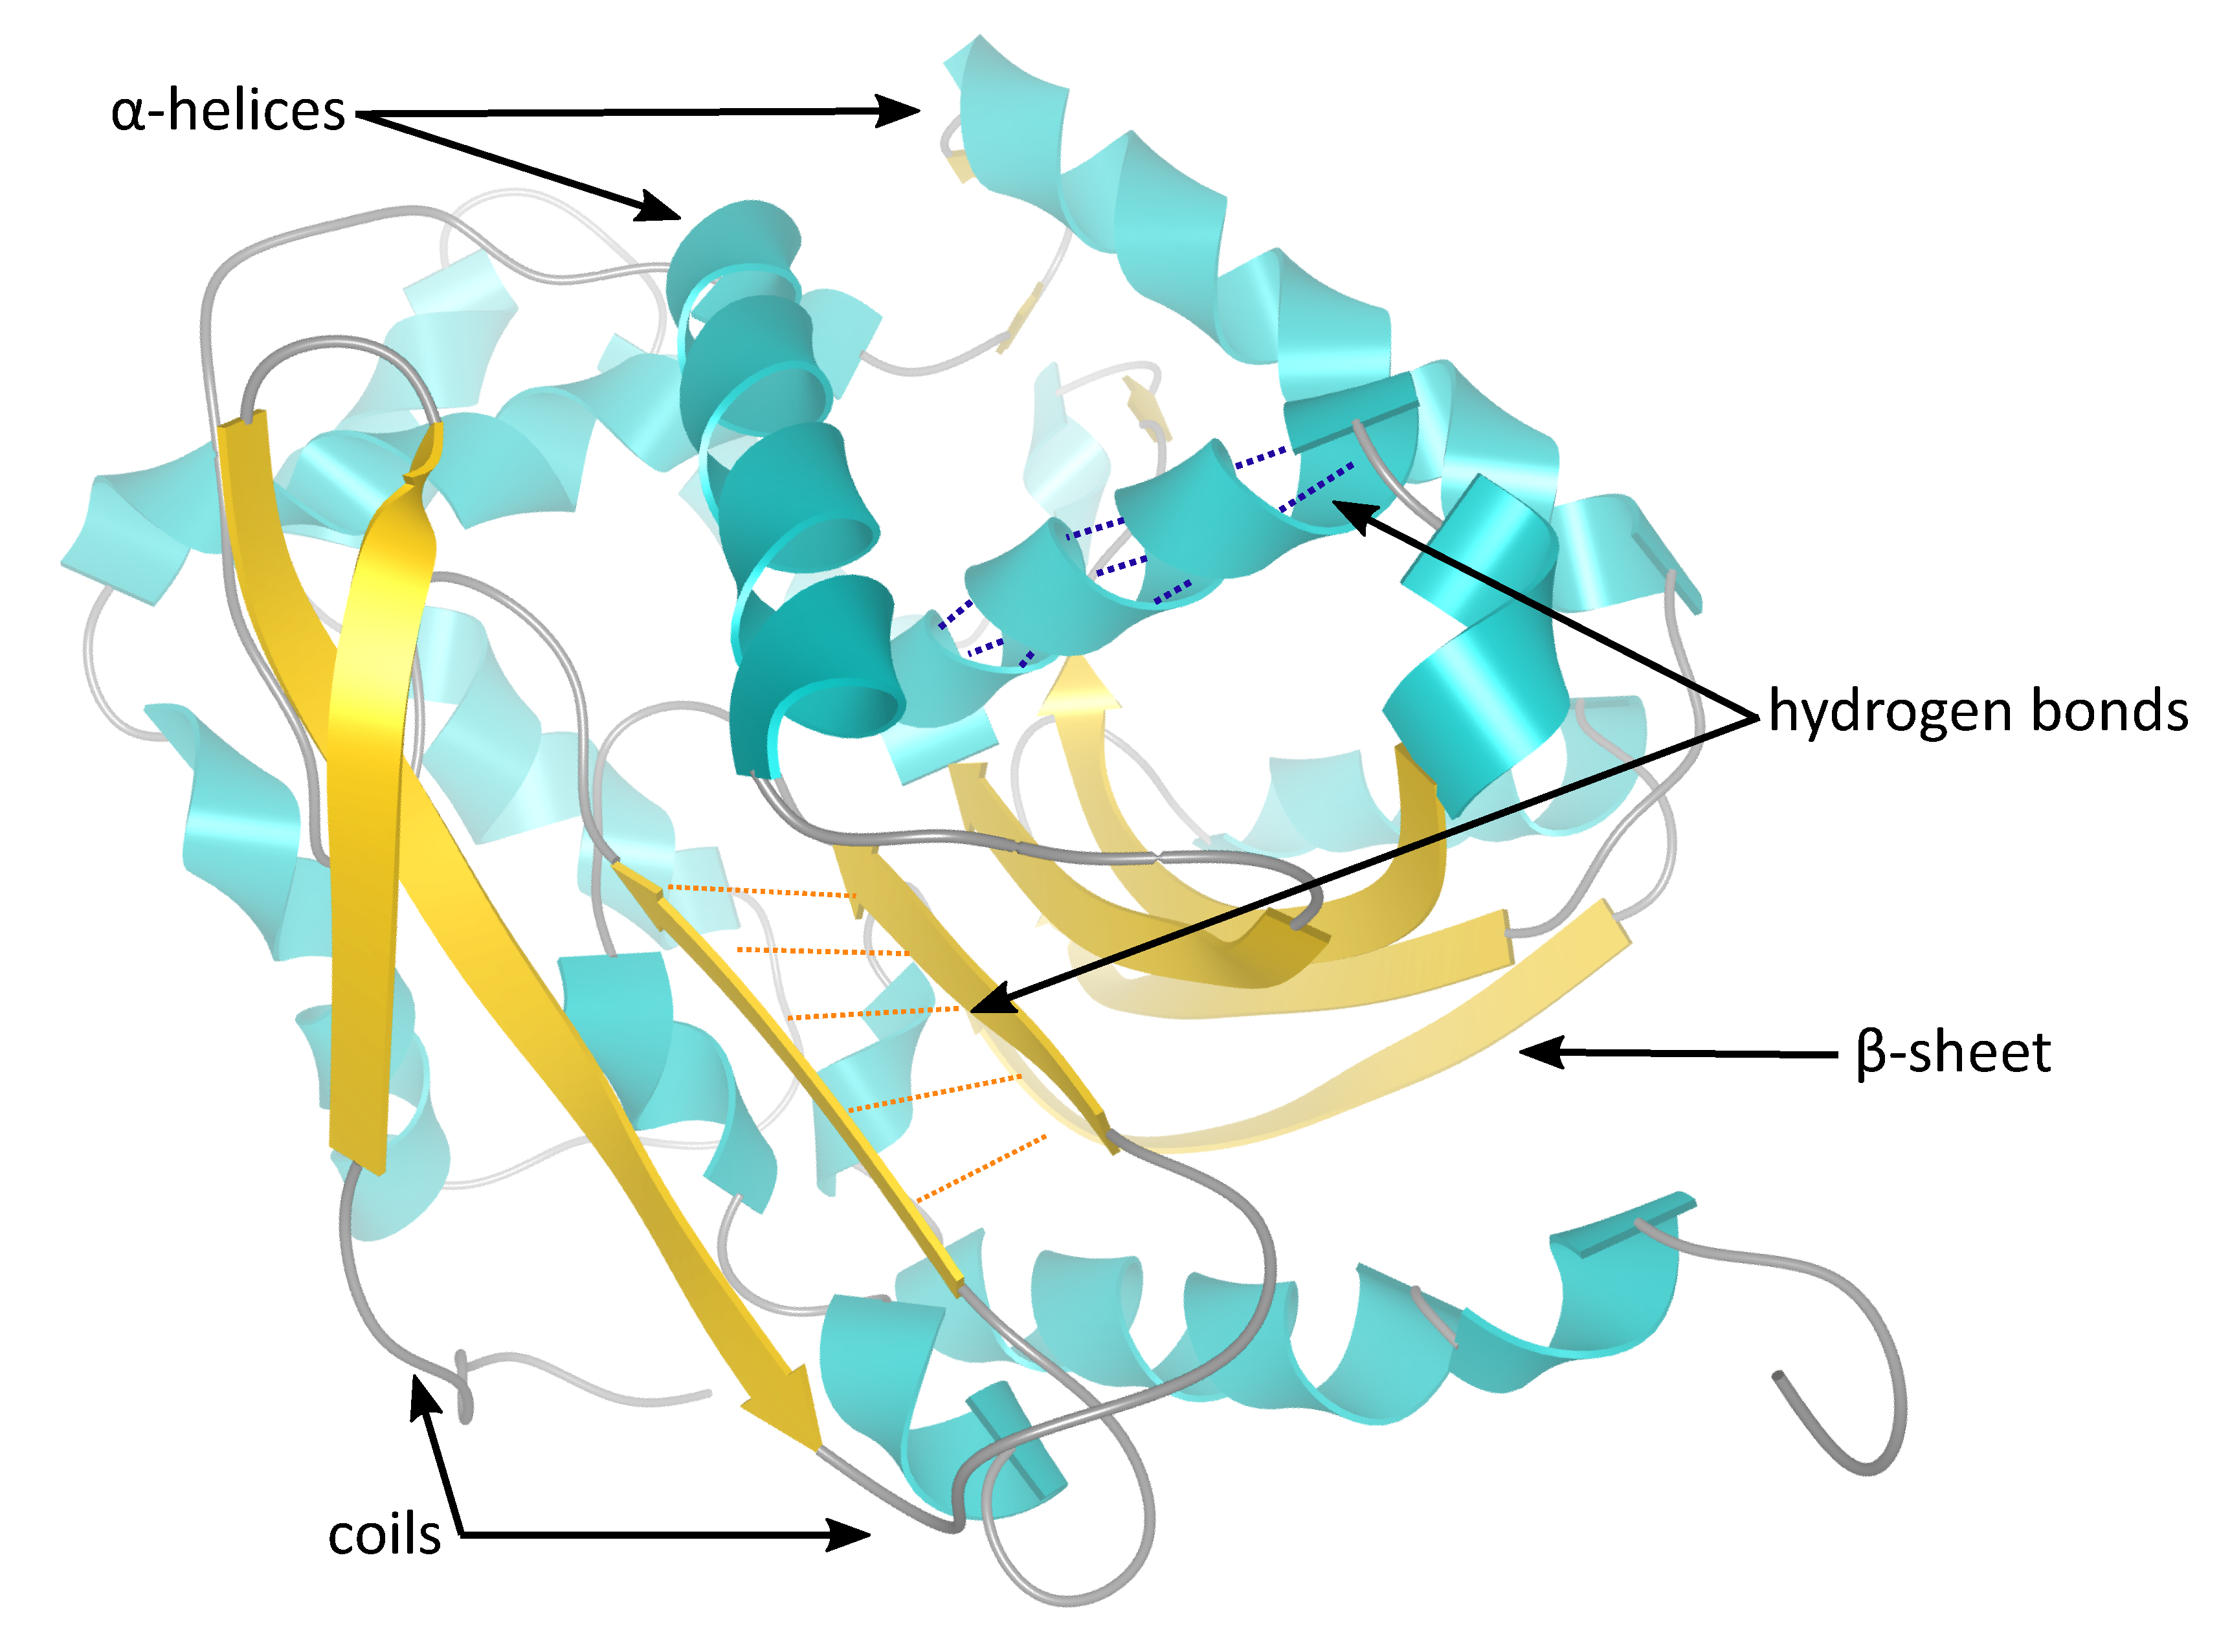
\includegraphics[width=.6\textwidth]{pictures/secondary.pdf} 
  \caption{Typical secondary structures of protein: $\alpha-helices$ (blue), $\beta-strands$ (orange) forming $\beta-sheet$ and \textit{coils}.}
  \label{Fig:secondary}
\end{figure} 

Various side chains of amino acid residues can interact together during the formation of protein. As a result, the secondary structures of the protein are bended and shaped into a  unique 3D structure until the protein attains its minimal energy state. This process is called \textit{protein folding} and it results in a \textit{tertiary protein structure}. The tertiary structure defines the complete spatial arrangement of atoms of one polypeptide chain. Interactions between amino acids of multiple polypeptide chains than define their \textit{quaternary protein structure}.

\section{Properties of Proteins}
Previous section described the process of protein attaining its 3D structure. This structure directly influences the way protein is behaving with regards to other molecules and its ability to function properly.

Example of this are the inner voids of the protein. When protein folds, there is naturally some empty space left inside. Depending on the shape of the space we classify four types of inner voids(figure \ref{Fig:voids}): \textit{cavities} -- void space buried deeply inside the protein,  \textit{tunnels} -- connecting cavities with surface of the protein, \textit{channels} -- passing through the whole protein and \textit{pockets} -- shallow protrusions on the surface of the protein.

\begin{figure}[H]
  \centering
  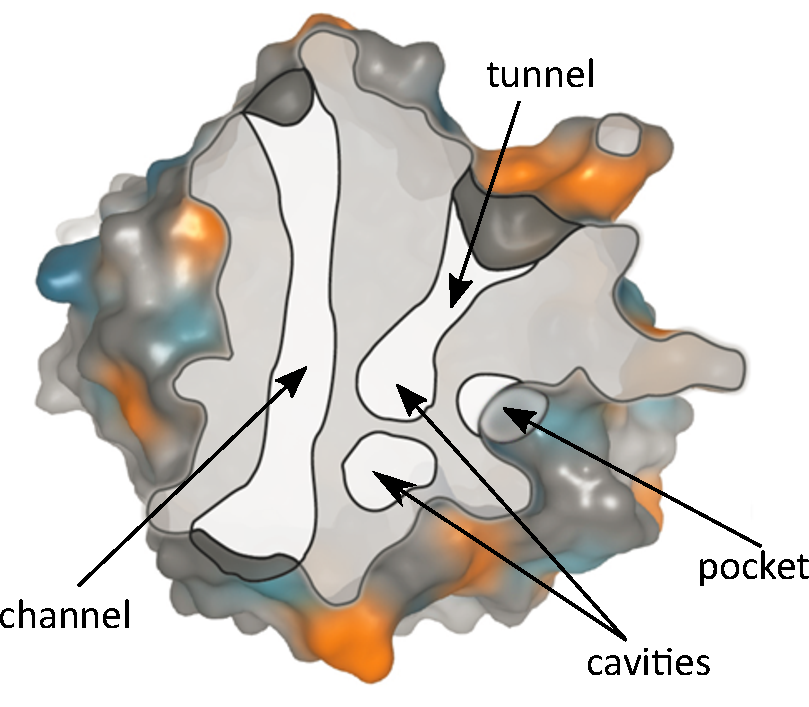
\includegraphics[width=.5\textwidth]{pictures/Voids.pdf} 
  \caption{Types of inner voids of protein.}
  \label{Fig:voids}
\end{figure}

These inner voids can significantly influence the reactivity of the protein since they contain \textit{active site}. Active site is a region of reactive amino acids, where other molecules can bind to protein and undergo a chemical reaction. This place is often buried deep inside the protein and its accessibility is thus limited by the size, shape but also physico-chemical properties of the voids leading to it.

\section{Protein-Ligand Interactions}
\textbf{Ligand}


In this thesis I will focus on two types of intermolecular interactions of proteins: a) protein-ligand interactions and b) protein-protein interactions. 

Protein-ligand interaction. This type of reaction occurs when a protein reacts with a small molecule called ligand. Here the aim
single ligand-protein pair, key lock priciple....

\section{Protein-Protein Interactions}